\documentclass[12pt,openright,twoside]{book}
\usepackage{graphicx}
\usepackage{geometry}
\usepackage{pdflscape}
\usepackage{natbib}
\usepackage{amsmath}
\usepackage{pdflscape}
%%\usepackage{tabu}
\usepackage{caption}
%%\usepackage{floatrow}
\usepackage{enumerate}
\usepackage{enumitem}
\usepackage{titlesec}
\usepackage{wrapfig}

\titleformat{\chapter}
  {\Large\bfseries} % format
  {}                % label
  {0pt}             % sep
  {\LARGE}           % before-code

\renewcommand{\figurename}{\textbf{Figure}}
\renewcommand{\tablename}{\textbf{Table}}
\newcommand{\HRule}{\rule{\linewidth}{0.4mm}}

\renewcommand{\contentsname}{{\Huge Table of Contents}}
\renewcommand{\chaptername}{{\Huge  }}
%\renewcommand{\thebibliography}{\Bibliografie}


\geometry{
 a4paper,
 total={210mm,297mm},
 left=25.0mm,
 right=25.0mm,
 top=25.0mm,
 bottom=30.0mm,
 }

 \setcounter{tocdepth}{3}
%level -1: part, 0: chapter, 1: section, etc.

\begin{document}

\begin{titlepage}
\begin{center}






\includegraphics[width=16cm]{./antet_L.jpg}



\vspace{4cm}



    \HRule \\[0.3cm]


    {\Large \textsc {Titlul tezei}}\\


  \HRule \\[1.1cm]

  \textsc{\large Lucrare de Licen\c{t}\u{a}}\\[4cm]

   \begin{flushleft} \large
    {Absolvent} \\[0.1cm]
    Luca Mircea MIHĂILESCU
   \end{flushleft}

   \begin{flushright} \large
    {Conduc\u{a}tor \c{s}tiin\c{t}ific} \\[0.1cm]
    Conf. Univ. Dr. Alexandru NICOLIN
   \end{flushright}


  \vfill

  % Partea de jos a paginii
 %% {\large \today}

 {\large Bucure\c{s}ti, 2020}

\end{center}

\end{titlepage}
\newpage
\vspace*{\fill}
\thispagestyle{empty}




\newpage
\thispagestyle{plain} \pagenumbering{roman}


\vspace*{36pt}

\begin{center}

{\LARGE \textbf{Cuv\^ant \^Inainte/Mul\c{t}umiri}}

\end{center}

\vspace{36pt}
Titlul acestuei Sectiuni este la alegere: Cuvant Inainte sau Multumiri; depinde ce doriti sa contina. Lorem ipsum dolor sit amet, consectetur adipisicing elit, sed do eiusmod tempor incididunt ut labore et dolore magna aliqua. Ut enim ad minim veniam, quis nostrud exercitation ullamco laboris nisi ut aliquip ex ea commodo consequat.\\

Lorem ipsum dolor sit amet, consectetur adipisicing elit, sed do eiusmod tempor incididunt ut labore et dolore magna aliqua. Ut enim ad minim veniam, quis nostrud exercitation ullamco laboris nisi ut aliquip ex ea commodo consequat.\\

Lorem ipsum dolor sit amet, consectetur adipisicing elit, sed do eiusmod tempor incididunt ut labore et dolore magna aliqua. Ut enim ad minim veniam, quis nostrud exercitation ullamco laboris nisi ut aliquip ex ea commodo consequat.\\

\vspace{40pt}


%%\noindent\textbf{NB} \textit{Mul\c{t}umiriile pot fi incluse aici, nu este necesar un capitol special }

\vspace*{\fill}
\newpage
\thispagestyle{empty} \vspace*{\fill} \tableofcontents

\setlength\parindent{0pt}



\setcounter{page}{0}

%% this comand remove indent

\newpage

 \pagenumbering{arabic}


\chapter{Introduction}
\label{intro}

Lorem ipsum\cite{book1} dolor sit amet \cite{book1,art1},  consectetur adipisicing elit, sed do eiusmod tempor incididunt ut labore et dolore magna aliqua. Ut enim ad minim veniam, quis nostrud exercitation ullamco laboris nisi ut aliquip ex ea commodo consequat..\\

Lorem ipsum dolor sit amet, consectetur adipisicing elit, sed do eiusmod tempor incididunt ut labore et dolore magna aliqua. Ut enim ad minim veniam, quis nostrud exercitation ullamco laboris nisi ut aliquip ex ea commodo consequat.
\\


Lorem ipsum dolor sit amet, consectetur adipisicing elit, sed do eiusmod tempor incididunt ut labore et dolore magna aliqua. Ut enim ad minim veniam, quis nostrud exercitation ullamco laboris nisi ut aliquip ex ea commodo consequat.\\

\begin{equation}
t=\frac{D{_{p}}}{D{_{0}}}
\label{eq1}
\end{equation}

\vspace{14pt}

unde: ${D{_{p}}}$ este doza total\u{a} acumulat\u{a} numit\u{a} paleodoza iar ${D{_{0}}}$ reprezint\u{a} doza anual\u{a} de radia\c{t}ii. Ecuatia in text se citeaza (\ref{eq1})\\

\begin{figure}
\centering
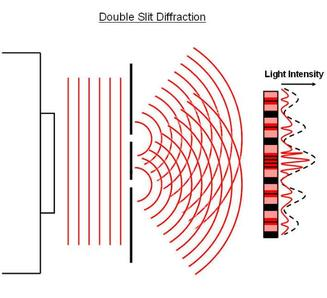
\includegraphics[width=7cm]{figure1.jpg}
\caption{\textit{{\small Legenda figurii}}}
\end{figure}

Lorem ipsum dolor sit amet, consectetur adipisicing elit, sed do eiusmod tempor incididunt ut labore et dolore magna aliqua. Ut enim ad minim veniam, quis nostrud exercitation ullamco laboris nisi ut aliquip ex ea commodo consequat.\\

\begin{figure}
 \centering
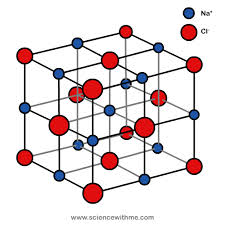
\includegraphics[width=7cm]{figure2.jpg}
\caption{\textit{{\small Legenda figurii}}}
\label{fig1}
\end{figure}

Figura in text se citeaza Figura (\ref{fig1}). Lorem ipsum dolor sit amet, consectetur adipisicing elit, sed do eiusmod tempor incididunt ut labore et dolore magna aliqua. Ut enim ad minim veniam, quis nostrud exercitation ullamco laboris nisi ut aliquip ex ea commodo consequat.\\

\chapter{Statistical Physics of Social Dynamics: A Brief Review}

-translation + tradition\\
The idea of a physical modeling of social phenomena is not at all a new one. In an 1825 essay, french philosopher Auguste Comte defines social physics as: "that science which occupies itself with social phenomena, considered in the same light as astronomical, physical, chemical, and physiological phenomena, that is to say as being subject to natural and invariable Laws the discovery of which is the special object of its researches."\cite{iggers_1959,comte_1825} He would later go on to refer to this new field as sociology.\\

\begin{table}[b]
\centering
\begin{small}
{\caption{\textit{Equivalence of thermodynamics terms to social science according to Mimkes' model of regular mixtures}}}
\begin{tabular}{ccc}

\hline\hline
Abbreviation  & Natural Science & Social science\u{a}      \\
\hline
A-B           & Alloys                  & Societies   \\
$x$           & atomic percentage       & size of minority (\%)  \\
              & \underline{Functions}   & \underline{Feelings} \\
$G$           & free enthalpy           & general happiness   \\
$T$           & temperature             & tolerance  \\
$E_{AA}$      & cohesive energy         & tradition, heritage\\
$E_{AB}>0$    & cohesive energy         & curiosity, love   \\
$E_{AB}<0$    & repelling energy        & distrust, hate  \\
$E=0$         & no cohesion             & apathy  \\
$\epsilon>0$  & attractive interaction  & sympathy  \\
$\epsilon=0$  & ideal solution          & indifference          \\
$\epsilon<0$  & repelling interaction   & antipathy  \\
              & \underline{State of alloys}         & \underline{State of Society}  \\
              & disorder, solubility    & integration  \\
              & solubility limit        & segregation  \\
              & phase diagram           & intermarriage diagram  \\

\hline
\end{tabular}
\end{small}
\end{table}

\section{The Ising Paradigm}
-Ising + voter model
\section{Cultural dynamics}
-cultural dynamics

\chapter{Model Setup}

In this thesis, I model opinion dynamics by using a Potts-like agent-based model, and the evolution of the network structure is performed by using a slightly modified version of Axelrod's model of dissemination of culture. This chapter provides the reader with a detailed description of the proposed model.\\

\section{Agent characteristics}

A directional network consisting of N agents is used. Each agent is represented by a vertex in the network, accompanied by a set of three features. These features are:\\

\begin{enumerate}
  \item \textbf{Vote:} a variable in the range of $v=0..n$, representing the agent's opinion. \textit{Votes} can be understood literally, as voting intention in an election, or, more generally, as an opinion subject to quick change in a social network.
  \item \textbf{Cultural vector:} a vector $\sigma=(\sigma_1,...,\sigma_F)$, with $\sigma_f=0,1,...,q$, representing an immutable set of cultural characteristics. Here culture is understood as, in Axelrod's words, "\textit{the set of individual attributes that are subject to social influence}".
  \item \textbf{Energy:} defined as $\epsilon_{i}=-J\sum_{j}\delta{v_i,v_j}$, where $j\in$ inneighbors, and $\delta$ is the Kronecker delta symbol. Note that this definition is akin to the Potts model Hamiltonian, with the difference that in this case spins are replaced by \textit{votes}.
\end{enumerate}

\vspace{14pt}

\section{Network rewiring}

Each step, an agent is selected for which, with a certain probability, an inneighbour will be removed and another added. Here, I referred to the transition probability defined by Axelrod for his model of dissemination of culture:\\

\begin{equation}
\omega_{i,j}=\frac{1}{F}\sum_{f=1}^{F}\delta_{\sigma_f(i),\sigma_f(j)}
\label{ax_trans_prob}
\end{equation}

\vspace{14pt}

However, this probability only grows when to cultural characteristics are \textit{identical}. In reality, beliefs are usually on a spectrum of intensity. For instance, a person with a belief $\sigma_f=3$ will find themselves more likely to interact with another with $\sigma_f=4$ rather than one with $\sigma_f=9$. Taking this into consideration, a new function $\eta$ can be devised:\\

\begin{equation}
\eta_{i,j}=1-\frac{1}{F}*\frac{1}{q}\sum_{f=1}^{F}|\sigma_f(i)-\sigma_f(j)|
\label{trans_prob}
\end{equation}

\vspace{14pt}

Using this revised probability, this stage in the time-step is defined by the following activities:\\

\begin{itemize}
    \item One agent $i$ is selected at random.
    \item Another agent $j$ that is not an inneighbour is selected randomly.
    \item With a probability $\eta_{i,j}$ an edge from $j$ to $i$ is added, and $i$'s energy $\epsilon_i$ is reevaluated.
    \item Now an agent $k$ is selected randomly from $i$'s inneigbours.
    \item With a probability $1-\eta_{i,j}$ the edge from $k$ to $i$ is removed, and $i$'s energy $\epsilon_i$ is reevaluated. 
\end{itemize}

\vspace{14pt}

It is immediately apparent that this rewiring procedure will lead to similar agents becoming more connected, and eventually forming hubs. This behaviour mirrors the echo-chamber effect observed in social media.\\

\section{Opinion dynamics}

Having rewired the network the selected agent's connections, it will now reconsider its \textit{vote}. This happens by attributing a new random vote to the agent, and reevaluating agent energy with the new vote. If the energy is lower, i.e. the agent's opinion is more in line with his influencers', then the new vote is kept. Otherwise, it will keep its new opinion with a certain probability, which is dependent on temperature (tolerance) $T$ and difference in energy $\Delta\epsilon=\epsilon_{new}-\epsilon_{old}$:\\

\begin{equation}
p=exp(-\frac{\Delta\epsilon}{T})
\label{switch_prob}
\end{equation}

\vspace{14pt}

\section{Overall execution procedure}

Putting the network rewiring part and the opinion dynamics parts together, the algorithm will go through the following procedure:\\

\textbf{Step 1: Generating initial population.} A data vector containing $N$ data structures is created, where each data structure contains the features described at section 2.1, with random votes and cultural vectors.\\

\textbf{Step 2: Network initialization.} A Barabási–Albert graph is initialized, growing by adding new vertices to $N_0$ initial vertices. Each new vertex is attached to $k$ different vertices already present in the system by preferential attachment.\\

\textbf{Step 3: Compute initial energy and vote distribution.} Compute energy for each agent, count vote distribution, then store the data in the log.\\

\textbf{Step 4: Select random agent.}\\

\textbf{Step 5: Network rewiring.} Perform the network rewiring procedure on the selected agent, recalculating $\epsilon$ and $E$ afterwards.\\

\textbf{Step 6: Opinion dynamics.} Perform the opinion dynamics procedure on the selected agent, recalculating $\epsilon$ and $E$ afterwards.\\

\textbf{Step 7: Advance to next step.} Advance the time step and go back to Step 4 until desired number of steps is reached.\\

\textbf{Step 8: Data export.} The generated data containing the $E$ time series, vote distribution over time and the final network form is exported.\\  

\subsection{Lorem ipsum}

Lorem ipsum dolor sit amet, consectetur adipisicing elit, sed do eiusmod tempor incididunt ut labore et dolore magna aliqua. Ut enim ad minim veniam, quis nostrud exercitation ullamco laboris nisi ut aliquip ex ea commodo consequat.\\

Lorem ipsum dolor sit amet, consectetur adipisicing elit, sed do eiusmod tempor incididunt ut labore et dolore magna aliqua. Ut enim ad minim veniam, quis nostrud exercitation ullamco laboris nisi ut aliquip ex ea commodo consequat.\\

Lorem ipsum dolor sit amet, consectetur adipisicing elit, sed do eiusmod tempor incididunt ut labore et dolore magna aliqua. Ut enim ad minim veniam, quis nostrud exercitation ullamco laboris nisi ut aliquip ex ea commodo consequat.\\

\vspace{40pt}


\noindent\textbf{NB} \textit{Citarile \^in text: }(Arhipova et al. 2000, Muhs 2013) sau [2,4]



\chapter{Titlul capitolului 3}

\section{Lorem ipsum }

\section{Lorem ipsum }

Lorem ipsum dolor sit amet, consectetur adipisicing elit, sed do eiusmod tempor incididunt ut labore et dolore magna aliqua. Ut enim ad minim veniam, quis nostrud exercitation ullamco laboris nisi ut aliquip ex ea commodo consequat. \\


\begin{table}[b]
\centering
\begin{small}
{\caption{\textit{Legenda tabelului}}}
\begin{tabular}{ccc}

\hline\hline
Proba & Ad\^ancimea (m) & Descriere sumar\u{a}      \\
\hline
PS I        & 4,5              & brun deschis   \\
L I         & 5,1              & brun           \\
L II        & 8,2              & brun deschis   \\
L III       & 9,1              & brun deschis  -  ro\c{s}ietic  \\
PS II           & 9,5              & brun         \\
L IV        & 10,1             & brun \^inchis - ro\c{s}ietic   \\
PS III      & 10,4             & brun \^inchis  \\
L V         & 10,9             & ro\c{s}u brun  \\
L VI        & 11,8             & ro\c{s}u brun  \\
PS IV       & 19,1             & ro\c{s}u brun  is\^inchis          \\
\hline
\end{tabular}
\end{small}
\end{table}




\subsection{Lorem ipsum }

Lorem ipsum dolor sit amet, consectetur adipisicing elit, sed do eiusmod tempor incididunt ut labore et dolore magna aliqua. Ut enim ad minim veniam, quis nostrud exercitation ullamco laboris nisi ut aliquip ex ea commodo consequat.\\

Lorem ipsum dolor sit amet, consectetur adipisicing elit, sed do eiusmod tempor incididunt ut labore et dolore magna aliqua. Ut enim ad minim veniam, quis nostrud exercitation ullamco laboris nisi ut aliquip ex ea commodo consequat.\\

Lorem ipsum dolor sit amet, consectetur adipisicing elit, sed do eiusmod tempor incididunt ut labore et dolore magna aliqua. Ut enim ad minim veniam, quis nostrud exercitation ullamco laboris nisi ut aliquip ex ea commodo consequat.\\

\subsection{Lorem ipsum }

Lorem ipsum dolor sit amet, consectetur adipisicing elit, sed do eiusmod tempor incididunt ut labore et dolore magna aliqua. Ut enim ad minim veniam, quis nostrud exercitation ullamco laboris nisi ut aliquip ex ea commodo consequat.\\

Lorem ipsum dolor sit amet, consectetur adipisicing elit, sed do eiusmod tempor incididunt ut labore et dolore magna aliqua. Ut enim ad minim veniam, quis nostrud exercitation ullamco laboris nisi ut aliquip ex ea commodo consequat.\\

Lorem ipsum dolor sit amet, consectetur adipisicing elit, sed do eiusmod tempor incididunt ut labore et dolore magna aliqua. Ut enim ad minim veniam, quis nostrud exercitation ullamco laboris nisi ut aliquip ex ea commodo consequat.\\


\chapter{Concluzii/Concluzii Generale}

Titlul acestui capitol este Concluzii daca nu exista concluzii partiale la sfarsitul fiecarui capitol sau Concluzii Generale in caz contrar. Lorem ipsum dolor sit amet, consectetur adipisicing elit, sed do eiusmod tempor incididunt ut labore et dolore magna aliqua. Ut enim ad minim veniam, quis nostrud exercitation ullamco laboris nisi ut aliquip ex ea commodo consequat.\\

Lorem ipsum dolor sit amet, consectetur adipisicing elit, sed do eiusmod tempor incididunt ut labore et dolore magna aliqua. Ut enim ad minim veniam, quis nostrud exercitation ullamco laboris nisi ut aliquip ex ea commodo consequat.\\

Lorem ipsum dolor sit amet, consectetur adipisicing elit, sed do eiusmod tempor incididunt ut labore et dolore magna aliqua. Ut enim ad minim veniam, quis nostrud exercitation ullamco laboris nisi ut aliquip ex ea commodo consequat.\\







\renewcommand{\contentsname}{References}
\renewcommand\bibname{References} %
\addcontentsline{toc}{chapter}{References}
\markboth{References}{References} %
\bibliographystyle{unsrt}
%
%\bibliographystyle{plain}

\bibliography{References}


\end{document}
